\section{Decentralized Unstructured Architectures}
\label{section:unstructured}

This section is dedicated to the unstructured P2P architectures. In the next
paragraphs,algorithms for tackling the topology mismatch problem on such
networks are discussed, analysed and categorised based on the use of the
overlay structure, message forwarding approach for peer communication and
techniques proposed for detecting proximity in order to optimise overlay
topology.

% TODO: READ A Near-Optimal Algorithm Attacking the Topology Mismatch Problem in
%Unstructured Peer-to-Peer Networks (This is an Approximation alg for Top-mis
%problem)

%%%%%%%%%%%%%%%%%%%%%%%%%%%%%%%%%%%%%%%%%%%%%%%%%%%%%%%%%%%%%%%%%%%%%%%%%%%%%%%%
%
% TODO: HOW CAN UNSTRUCTURED SCHEMES BE REFINED
%
%For this reasons, efforts have been placed for optimizing the efficiency of
%decentralized unstructured peer-to-peer networks. Research mainly focuses on
%\begin{inparaenum}[\itshape i\upshape)]
%  \item reducing unnecessary, redundant communication traffic, and
%  \item exploiting physical locality to reduce communication response.
%\end{inparaenum}
%The goal can be achieved at, both, the application-level network as well as the
%underlying physical one. In the first case by refining the message relay
%techniques, while in the second one, by adaptively reconstructing the
%application network to map as well as possible to the the physical network.
%
%%%%%%%%%%%%%%%%%%%%%%%%%%%%%%%%%%%%%%%%%%%%%%%%%%%%%%%%%%%%%%%%%%%%%%%%%%%%%%%%


\subsection{Algorithms for Unstructured Architectures}


%###############################################################################
%###############################################################################
%       BROADCAST OPTIMISATION
%###############################################################################
%###############################################################################


%%%%%%%%%%%%%%%%%%%%%%%%%%%%%%%%%%%%%%%%%%%%%%%%%%%%%%%%%%%%%%%%%%%%%%%%%%%%%%%%
\subsubsection{Improving search in peer-to-peer networks}

\begin{figure}[ht]
\centering
\subfigure[Iterative deepening with three levels.] {
  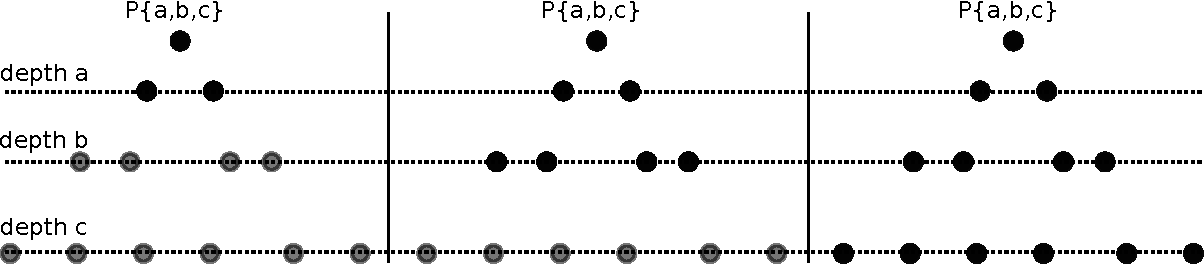
\includegraphics[scale=0.4]{img/algorithms/iterative_deepening}
  \label{figure:dbfs:iterdeep}
}\qquad\qquad
\subfigure[Directed BFS.] {
  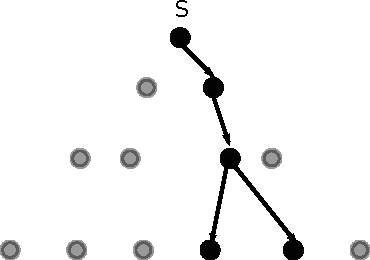
\includegraphics[scale=0.4]{img/algorithms/directed_bfs}
  \label{figure:dbfs:dbfs}
}\qquad\qquad
\subfigure[Local indices with radius size equal to $2$.] {
  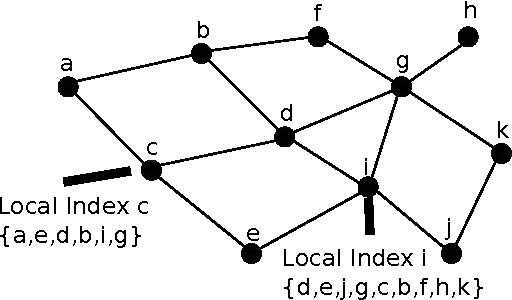
\includegraphics[scale=0.4]{img/algorithms/local_indices}
  \label{figure:dbfs:localindx}
}
\caption{Improving search in P2P networks}
\label{figure:dbfs}
\end{figure}

\cite{yang_improvep2psearch_2002} proposes an easy to implement and practical
solution to the inefficiency of Gnutella's ``blind flooding'' approach. The
paper introduces three different forwarding methods, namely \emph{iterative
deepening}, \emph{directed BFS}, and \emph{local indices}.

In iterative deepening (see Figure~\ref{figure:dbfs:iterdeep}), the search is
performed on a BFS tree with multiple preset depths. The depth limit is
iteratively increased by the source node for each query, based on the quality of
the results. The source node may issue a new request with increased depth limit
that will trigger the nodes at the last depth level to resume the search. The
iterative approach avoids restarting the whole search process from scratch at
each iteration and reduces the load of the nodes on the upper levels of the
tree. Its major drawback is the delay between successive iterations, as the
source node needs to examine the results at each iteration before deciding to
quit or resume the query.

The directed BFS, as shown in Figure~\ref{figure:dbfs:dbfs}, tries to avoid this
delay by forwarding the query messages only to a selected set of neighbours, in
which the selection criteria varies from the number of results received
previously, distance in terms of hops, bandwidth, or the query load of the
neighbour.

% TODO: local indices is a cache based algorithm so maybe we have to put a
% reference to the respective section???
In local indices, as shown in Figure~\ref{figure:dbfs:localindx}, each node
indexes data within a radius of $r$ hops and uses this local index to answer
queries on behalf of them without generating additional traffic. Local indices
greatly reduce the aggregate bandwidth usage of the network and improves query
efficiency, however, updating the indices in cases with frequent node joins and
leaves introduces a serious overhead to the system if the radius is kept broad.

%%%%%%%%%%%%%%%%%%%%%%%%%%%%%%%%%%%%%%%%%%%%%%%%%%%%%%%%%%%%%%%%%%%%%%%%%%%%%%%%
\subsubsection{Gia}
\emph{Gia} \cite{chawathe_gia_2003} is an effort to solve the scalability
problem of the unstructured P2P file sharing systems, in particular Gnutella.
The main novelty in the design of Gia is the replacement of the blind flooding
approach of Gnutella with random walks \cite{lv_randomwalks_2002}. Although
random walks is a step in the right direction, issuing only a single copy of the
query within the network reduces the search scope, thus affecting negatively the
success rate of the query.  In order to overcome this limitation, Gia introduces
a token-based flow control mechanism, which is essentially an intelligent flow
control algorithm that gradually redirects the queries to nodes which are more
likely to answer. In order to prevent overloading of nodes with query requests,
Gia uses a token-based flow control algorithm in which each node announces the
number of query requests it can handle in terms of tokens to its neighbours, so
that neighbours only forward query requests to nodes that they previously
received tokens from. Gia also acknowledges the heterogenity in peer bandwidth,
processing power, disk speed, etc, of the nodes in P2P networks and uses this
information when connecting nodes to each other and by using a topology
adaptation algorithm, Gia ensures that high capacity nodes have high degrees and
low capacity nodes are within short proximity to high capacity ones.
% TODO: THIS FOLLOWING REMARK SOUNDS LIKE THE ALGORITHM SHOULDN'T BE IN THIS
%       SURVEY AFTER ALL!!
Although the topology adaptation algorithm Gia uses improves the scalability of
the network, it does not help much in solving the topology mismatch problem,
since it does not consider the underlying physical topology.

% TODO: from the following (commented out) design components of Gia has one
% part that falls into topology adaptation, one part on forwarding optimisation
% and one part on 

%
%More specifically, there are four key components in the design of
%\emph{Gia} which are summarized bellow:
%\begin{enumerate}
%  \item A \emph{dynamic topology adaptation} protocol that puts
%participating nodes within short reach of high capacity nodes so that these
%\emph{high-degree} nodes, which due to their high connectivity receive most of
%the queries, actually have the capacity to handle them.
%  \item An \emph{active flow control} scheme is used to avoid overloaded
% hot-spots. Heterogeneity is detected and flow control tokens are given to
%nodes based on the available capacity.
%  \item Every node maintains pointers to to the content that is offered by
% their immediate neighbours, creating a \emph{one-hop replication} of pointers,
%scheme.
%  \item A \emph{search protocol} based on random walks, that is biased towards
% directing queries to high-capacity nodes that are typically best able to
%answer these queries.
%\end{enumerate}
%

%%%%%%%%%%%%%%%%%%%%%%%%%%%%%%%%%%%%%%%%%%%%%%%%%%%%%%%%%%%%%%%%%%%%%%%%%%%%%%%%
\subsubsection{Distributed Cycle Minimization Protocol (DCMP)}
We have already discussed that blind flooding mechanism broadcasts messages with
no real targeting, many times to a direction far from the path that can
ultimatelly fullfil the query request. Another problem with topology unaware
systems is the duplication of messages due to cycles, even along the correct
forwarding path. The authors of \cite{zhu_dcmp_2008} fucused on that exact
deficiency of overlay networks and introduced Distributed Cycle Minimization
Protocol (DCMP), a dynamic, fully distributed method to remove cycles without
sacrificing overlay connectivity, resilience and other important properties of
unstructured architectures by avoiding a hierarchical organisation of peers. In
DCMP, once a cycle is detected, the most powerful node in that cycle is
elected as the \emph{Gate Peer} and the cycle is then broken at a strategic
place so that it will result in the minimisation of the distance between the
Gate Peer and all other nodes that participated in that cycle. The process
is managed by using two special message types namely \emph{Information
Collection (IC)} and \emph{Cut Message (CM)}. One disadvantage of DCMP is that
since the distance a forwarded message can travel is limited by the TTL value,
which is practically $7$ in most cases DCMP cannot detect cycles formed by more
than 7 peers. Even though cycle elimination improves the network performance, it
does not actually solve the topology mismatch problem.

%
%\subsection{Distributed Cycle Minimization Protocol}
%
%\paragraph{}
%The first step after detecting a duplicate message by some peer is to gather
% information from all peers in the cycle using a new type of control message
%called \emph{Information Collecting Message} or \emph{ICM}. ICM contains:
%\begin{inparaenum}[\itshape i\upshape)]
%  \item a \emph{GUID}\footnote{Globally Unique IDentifier assigned to every
% query message generated by any node.} field same as the one of the duplicate
%message,
%  \item \emph{DetectionID} field which represents the direction of the
% connection where the duplicate was identified\footnote{This ensures the
%uniqueness of the ICM messages because as it travels through many cyclic paths,
%multiple peers will detect the duplicates and initiate an ICM message.}, and
%  \item \emph{Node Information Vector (NIV)} which contains information
% (bandwidth, CPU power, etc) about peers that propagated the ICM.
%\end{inparaenum}
%
%\paragraph{}
%Suppose $A$ detected the duplicate as depicted in Figure~\ref{figure:dcmp}. It
% then emits an ICM to $B$ and $F$, that initially contains information only
%about itself. Each peer that receives the ICM, appends its information and
%propagates it along the reverse path of the original message. Since two copies
%of ICM are sent, at some point, a peer, say peer $D$, will receive a duplicate
%ICM. Using the information in the NIVs of the ICMs, $D$, decides to cut (for
%example) the EF connection. To inform the other peers about its decision, it
%emits a \emph{Cut Message (CM)} which contains the GUID and DetectionID of the
%corresponding ICM and an additional field that identifies the connection to be
%cut. $D$, then, forwards the CM in the reverse directions from where the ICM
%arrived. Similarly CMs received by any peer are propagated toward the reverse
%path of the corresponding ICM. Eventually, either peer $E$ or peer $F$ will
%receive the CM and cut the connection, thus eliminating the cycle.
%
%Receiving a duplicate ICM denotes the existence of a cycle. The opposite is not
% true though. For example, if the cycle contains $2 \times TTL$ edges, it will
%not be detected, because the ICM messages will be discarded before they locate
%it. There is a tradeoff between preserving the connectivity of the network and
%minimizing the duplicates that makes such a possibility to be safely ignored.
%
%\begin{figure}
%\centering
%  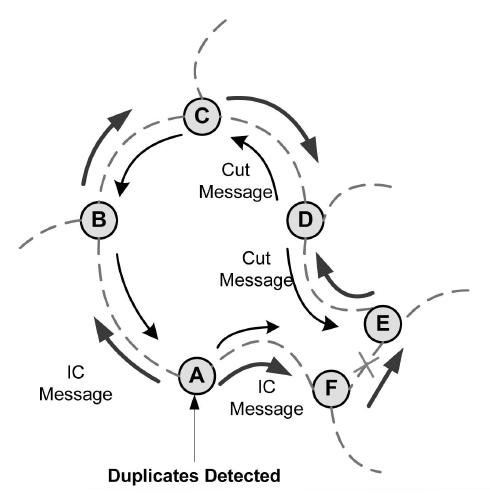
\includegraphics[scale=0.4]{img/dcmp.jpeg}
%\caption{Cycle elimination methods in DCMP}
%\label{figure:dcmp}
%\end{figure}
%
%\paragraph{}

%
% TODO: SOME DISCUSSION
%
%Actually, the duplicate packet problem seems to hurt more the active nodes;
%those with higher capacities and bandwidth that contribute the most to the
%network.
%Experiments in \cite{zhu_dcmp_2008} showed that DCMP incurs a lower delay,
% returns more results and decreases the number of duplicate messages by 22\%,
%compared to LTM. Additionally DCMP has one to two orders of magnitude less
%overhead, because it adopts a more ``LAZY'' approach than broadcasting control
%messages periodically like LTM does.
%

%###############################################################################
%###############################################################################
%###############################################################################
%       CACHING
%###############################################################################
%###############################################################################
%###############################################################################

%%%%%%%%%%%%%%%%%%%%%%%%%%%%%%%%%%%%%%%%%%%%%%%%%%%%%%%%%%%%%%%%%%%%%%%%%%%%%%%%
\subsubsection{Replication Strategies in Unstructured Peer-to-Peer Networks}
\cite{Cohen02} aim to improve the inefficient blind search algorithm by
replicating the data in a P2P network. The main intuition behind the
idea of replication, or using cached copies, is that as the number of copies for
each item increases in the network, it would be easier for a search algorithm,
even a random one, to locate these items. In order to analyse the feasibility of
such an approach, the authors investigate three different replication
strategies, namely uniform, proportional, and square root allocation. In the
uniform model, the copies of items are uniformly replicated in the network,
while in the proportional model, the items are replicated based on their query
rate, so that frequently queried items are replicated more. The square root
allocation is a strategy proposed in this paper, which is a model between the
uniform and proportional allocation.  In order to evaluate the outcome of the
replication models, the overall costs of successful and unsuccessful searches in
the network are compared. Results argue that the uniform allocation model
minimizes the maximum search size, therefore reduces the time spent on an
unsuccessful search. The proportional model, on the other hand, promotes the
more frequently queried items by replicating them more, therefore decreases the
search time for popular items, but suffers when needing to locate the rare
items. The authors also claim that the expected successful search size is the
same for uniform and proportional models, and any approach between them would
behave much better. Therefore they propose the square root allocation approach,
which is a replication strategy that minimizes the expected search size of
successful queries in P2P networks.

%%%%%%%%%%%%%%%%%%%%%%%%%%%%%%%%%%%%%%%%%%%%%%%%%%%%%%%%%%%%%%%%%%%%%%%%%%%%%%%%
\subsubsection{Tracing a large-scale Peer to Peer System: an hour in the
life
of Gnutella}
% TODO: This looks better as an analysis for the unstructured networks in
% general and specifically for caching, so it doesn't seem to contribute any
% new approach.... At least we do not present anything here. Maybe we need to
% revisit the paper itself once more
\cite{Markatos02} analyses Gnutella network traffic traces and by concluding
there is locality among query requests, proposes a caching algorithm that tries
to exploit these findings . The analysis of the trace data reveals other
important facts about the structure of the Gnutella network and the query data.
One significant observation is that the geographic locations of clients do not
have a correlation with the number of query requests they receive. This is an
obvious result of the topology mismatch problem caused by the overlay structure
of the Gnutella network. Gnutella's traffic is observed to be bursty both for
query requests and query responses, even in longer intervals. It is observed
that a peer receives 50 query messages per second on average! Moreover nine out
of ten queries do not generate any response due to the inefficient design of
the Gnutella network. When developing a caching system to exploit locality,
applying an approach similar to web caching does not fit well with P2P systems.
Caches in P2P systems not only have to consider the query string, but also
the TTL value, the source of the query, and the time of the query as well.  In
general, even though optimum caching is hard to achieve, it is reported that
it improves the overall performance of the Gnutella network.


%###############################################################################
%###############################################################################
%###############################################################################
%       OVERLAY OPTIMISATION
%###############################################################################
%###############################################################################
%###############################################################################

%%%%%%%%%%%%%%%%%%%%%%%%%%%%%%%%%%%%%%%%%%%%%%%%%%%%%%%%%%%%%%%%%%%%%%%%%%%%%%%%
\subsubsection{Narada}

\begin{figure}[ht]
\centering
\subfigure[Underlying network with edge costs.] {
  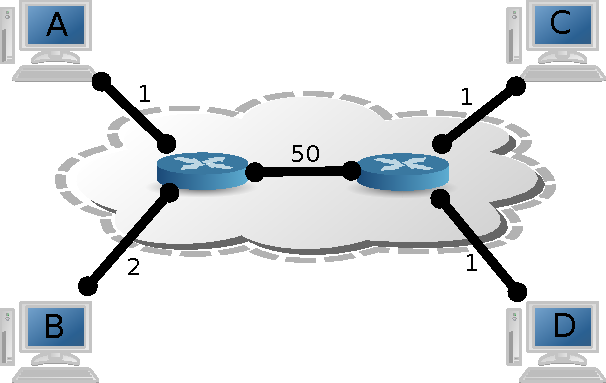
\includegraphics[scale=0.4]{img/algorithms/narada}
  \label{figure:narada:underlying}
}\qquad\qquad
\subfigure[Peer A sends a message to the rest using regular broadcast.] {
  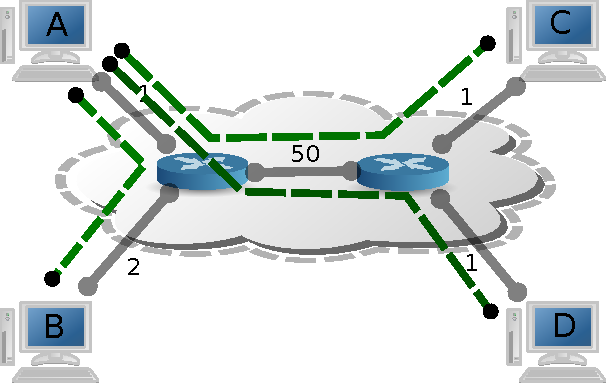
\includegraphics[scale=0.4]{img/algorithms/narada2}
  \label{figure:narada:regu}
}\qquad\qquad
\subfigure[Peer A sends a message to the rest using end system multicast.] {
  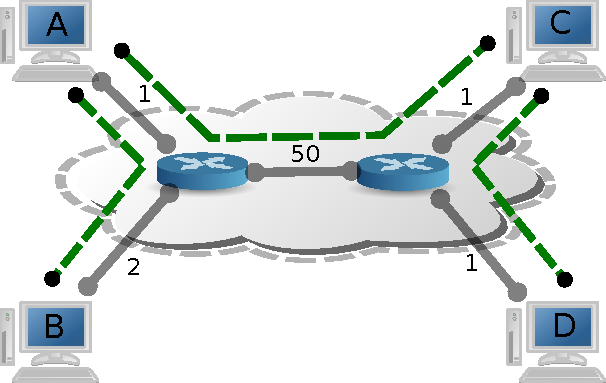
\includegraphics[scale=0.4]{img/algorithms/narada3}
  \label{figure:narada:multicast}
}
\caption{A visualisation of the Narada protocol.}
\label{figure:narada}
\end{figure}

\emph{Narada} \cite{chu_esm_2000,chu_esm_2001,chu_esm_2002} is a generic
protocol for creating self-adapting overlay networks, that can achieve
application-layer multicast communication without requiring IP multicast
infrastructure at the network layer\footnote{
  IP multicast is the term reffering to the method of sending IP datagrams to a
  group of receivers in a single transmission. Even though the method is
  available some years now, IP multicast has not taken off as anticipated since
  many believe that it violates the stateless design of the current Internet.
  For this reason it is widely deployed in contained environments like
  enterprises (i.e. IPTV applications - distance learning, video conferencing),
  commercial stock exchanges, and multimedia content delivery networks.
}. Although it was not originally designed as a P2P system nor can be considered
scalable in the contemporary sense of the term, Narada is considered pioneering
(maybe along with \emph{Scattercast} \cite{chawathe_scattercast_2000}) in that
it was the first to consider the feasibility of overlay-based, application
layer, services over the Internet that can take into account bandwidth and
latency properties of the physical underlying infrastructure. Additionally,
authors realised the inefficiency caused by the topology mismatch problem and
tried to encounter it by building a richer connected graph, called a
\emph{mesh}, and building per source minimum spanning trees\footnote{
  ENarada \cite{li_enarada_2008} used Gossip protocol for the construction
}
as shown in Figure~\ref{figure:narada}. They also keep the graph and the trees
dynamically updated while nodes continue to join and leave the network.
Moreover, the protocol tries to ease the physical link stress, the overall
resource usage and the relative delay among end systems. Unfortunately, the most
imporpant limitation of Narada is that although it works reasonably well for
small groups, it does not scale well for larger networks, therefore it is not
suitable for, potentially very large, P2P file sharing application networks.

%%%%%%%%%%%%%%%%%%%%%%%%%%%%%%%%%%%%%%%%%%%%%%%%%%%%%%%%%%%%%%%%%%%%%%%%%%%%%%%%
\subsubsection{Adaptive Overlay Topology Optimization (AOTO)}
\emph{Adaptive Overlay Topology Optimization (AOTO)} \cite{liu_aoto_2003} is one
of the first attempts, along with Narada, to address the topology mismatch
problem. AOTO is a distributed algorithm that works in two steps, namelly
\emph{Selective Flooding} and \emph{Active Topology} to optimize the usage of
the underlying physical resourses. In \emph{Selective Flooding} a minimum
spanning tree is built among each peer and its immediate neighbours so that
queries are not flooding the whole network and at the same time without
shrinking the search scope. During \emph{Active Topology}, the overlay
links are revised so that they depict the physical network topology as close as
possible. This is done independently, by each peer by replacing non-flooding
neighbours, with closer nodes. Picking a replacement out of these non-fooding
neighbours follows a random policy (called \emph{Randomized AT} algorithm in the
paper's context). For these steps a peer needs to keep track of communication
costs to all its neighbours (e.g. the network delay) as well as between any
pair of neighbours (meaning also that additional, cost probing, message types
need to be added to the Gnutella protocol). Whenever a new neighbour cost table
is received or there is a change of neighbours, the source peer has to
re-calculate the multicast tree and apply the randomized AT algorithm.

%\paragraph*{Selective Flooding (SF)}
%
% TODO: I DON'T REMEMBER WHY THE FOLLOWING IS MENTIONING LTM WHICH IS ANOTHER
%       ALGORITM. MAYBE THIS CAN BE USED AS A PART OF DISCUSSION AND/OR
%       COMPARISON OF AOTO AND LTM
% TODO: EDIT: LTM SEEMS A MISTAKE HERE BETTER NOT USE IT FOR DISCUSSION (THIS
%             IS AOTO)
%LTM's SF effectiveness has be proven to be detached from the different physical
% or overlay topologies. On the other hand, SF is more effective with large
%number of logical neighbours. It can reach an average optimization rate of 87.4
%percent on a logical topology with an average of 30 logical neighbours.
%
%\paragraph*{Active Topology (AT)}
%
%Different numbers of average logical neighbours has little to do with the
% effectiveness of AT. If the source has $n$ non-flooding peers, there are $n$
%potential neighbour replacements. The overhead to exhaust all $n$ possible
%replacements can be high, so in practice, after each replacement the source
%peer can decide whether it needs to find another candidate peer. This is done
%by computing the cost improvement ratio greater than some predefined
%termination threshold. The larger the threshold, the slower, in the number of
%optimization steps, the reduction of the normalized average distance. As a
%whole the average response time is significantly reduced when more optimization
%steps taken.

%%%%%%%%%%%%%%%%%%%%%%%%%%%%%%%%%%%%%%%%%%%%%%%%%%%%%%%%%%%%%%%%%%%%%%%%%%%%%%%%
\subsubsection{Adaptive Connection Establishment (ACE)}
\emph{Adaptive Connection Establishment (ACE)} \cite{liu_ace_2004} builds an
overlay multicast tree among each source node and the peers within a certain
diameter from the source peer and optimizes the neighbour connections that are
not in that tree. To achieve that it calculate cost between nodes using network
delay as a metric. Each peer probes the costs with its immediate logical
neighbours and forms a \emph{neighbour cost table (NCT)} using a special
routing message type. Two neighbouring peers exchange their NCTs in order for
every peer to obtain the cost between any pair of its local neighbours forming a
small overlay topology. Moreover, based on obtained NCTs a minimum spanning tree
among each peer and its immediate neighbours is built. Ultimately, physically
far away neighbours are replaced by physically close ones. Specifically, a peer
$S$ probes the distance between one of its non-flooding neighbour's neighbour,
say $G$ and $H$ respectively. Assuming that the link to the neighbour's neigbour
($SH$) is smaller that that of the neighbour ($SG$), the later is cut and a new
connection is established. In the oposite situation where $SG$ is smaller than
$SH$ then if $SH$ is smaller that $GH$ then $H$ is preserved as $S$'s new
neighbour. In the case where $SH$ is larger than $SG$ and $GH$, no connection
will be established and $S$ will continue probing another neighbour's neighbour.
The above optimisation is conducted within $1$-neighbour closure (among its
source peer and all its direct neighbours) but the scope can be extended. The
larger the scope, the better topology matching improvement but also the greater
the computational overhead.

%
% TODO: SOME DISCUSSION
%
%Simulations in \cite{liu_acesims_2004} show that the average scope of each
% query to cover the same scope of nodes is reduced by about 65 percent without
%losing any autonomy feature, while the average response time can be reduced by
%35 percent. Larger diameter topologies lead to better topology optimization
%rate but also to higher communication and computation overhead. It was also
%found that it is more effective in higher connectivity dense topologies.
%Compared to LTM, it comes short of convergence speed. In
%\cite{ni_mismatch_2004} shows reduction of both total traffic (90 percent) and
%response time (80 percent) to message queries without shrinking the search
%scope. SBO, on the other hand, achieves approximately 85 percent reduction on
%traffic cost and about 60 percent reduction on query response time. Last but
%not least, it is concluded that work must be done on incorporating a more
%sophisticated selection policy for candidate non-flooding peers.
%

%In \emph{Adaptive Connection Establishment (ACE)} \cite{liu_ace_2004}, the
%authors extend the idea of AOTO by introducing optimizations based on the
%depths of the minimum spanning trees. But since the network delay is not
%always a reliable estimation method to detect the physical location of peers,
%the algorithm still suffers from the discrepancies caused by mislocated nodes.

%%%%%%%%%%%%%%%%%%%%%%%%%%%%%%%%%%%%%%%%%%%%%%%%%%%%%%%%%%%%%%%%%%%%%%%%%%%%%%%%
\subsubsection{Location-aware Topology Matching (LTM)}
\emph{Location-aware Topology Matching (LTM)} \cite{liu_ltm_2004} proposes a
method to optimize the overlay structure of the P2P network based on the
physical topology. To achieve this, peers issue special messages called
\textit{TTL-detector}s with TTL values of 0 and 1 so that the receiving peers
discover one- and two-hop neighbour sets ($N$ and $N^2$ respectively) around
them and calculating communication costs. Calculation is achieved through
timestamp checking, so clocks must be synchronised. The latency information
gathered is later used to evolve the overlay network into a more efficient one,
without reducing the search scope. Each node examines the latency information
among his direct neighbours and those with larger latency are put in to a
will-cut list where they remain for a certain period of time until when they are
ultimatelly cut and recorded to the peer's cut list. Thus, low productive
connections are dropped and replaced by more efficient ones, reducing the
latency on the overall network. Although LTM improves the overall efficiency of
the P2P network, it does not actually use real physical topology information,
just latency metrics, therefore it does not offer a guaranteed safety net for
the topology mismatch problem.

%
% TODO: SOME DISCUSSION
%
%\paragraph*{Low productive connection cutting}
%There are three cases for any peer $P$ who receives $d(i, S, v)$ multiple
% times:
%\begin{inparaenum}[\itshape i\upshape)]
%  \item $P$ receives both $d(i, S, 1)$ and $d(i, S, 0)$
%  \item $P$ receives multiple $d(i, S, 0)$s from different paths, and P
% randomly chooses to process one
%  \item $P$ receives one $d(i, S, 1)$ and multiple $d(i, S, 0)$s, and $P$
% processes $d(i, S, 1)$ and one randomly selected $d(i, S, 0)$
%\end{inparaenum}
%If the link with the largest cost is found and is a direct neighbour then the
% connection is put in a will-cut list and stays there for a certain period of
%time. If it is not, then it is handled by other peers. After that period,
%connections are cut and recorded to $P$'s cut-list.
%
%\paragraph*{Source probing}
%For a peer $P\in(N^2(S) - N(S))$ who receives only one $d(i, S, 0)$, the cost
% of $PS$ is obtained (with list look-up or probing). Then $P$ compares it with
%the cost from each hop and if $PS$ has the largest cost, $P$ will not keep this
%connection, while otherwise the connection will be created.
%
%\paragraph{}
%Supposing $n$ is the number of peers, $c_n$ is the average number of neighbours
% and $c_e$ is the average cost of logical links, then in the flooding-based
%search the traffic incurred by one query from an arbitrary peer in a
%peer-to-peer network is $O(n)$. As observed in the Gnutella network
%\cite{sripanidkulchai_gnutella_2001}, each peer issues $0.3$ queries per minute
%in average, thus the per minute traffic incurred by the network with $n$ peers
%is $O(n^2)$. Because each $d(i, S, v)$ has a TTL of $2$ in each source peer,
%the traffic for one time LTM optimization in all peers is at most $2nc_n^2c_e$.
%If each peer uses LTM $k$ times per minute, the total traffic incurred is
%$2knc_n^2c_e$. Simulation shows the best value for $k$ is $2$ or $3$. So, the
%traffic overhead caused by LTM to the network is $O(n)$.
%
%TTLj-detectors, with $j > 2$, would detect and break cycles with more than 4
% links. LTM though, does not use such detectors because detector-flood traffic
%would increase significantly, and cut links between two end-peers, could cause
%queries initiated by them to traverse a path much more expensive than the cost
%on the the cut link.
%
%\paragraph{}
%LTM disadvantages are
%\begin{inparaenum}[\itshape i\upshape)]
%  \item disagreement of measured delay due to unsynchronized clocks causes
% problems when deciding the cut positions, which can influence the network
%connectivity, and
%  \item the network delay metric mainly focuses on disabling the connections
% between peers physically far away without considering the shortcuts created by
%powerful peers.
%\end{inparaenum}
%

%%%%%%%%%%%%%%%%%%%%%%%%%%%%%%%%%%%%%%%%%%%%%%%%%%%%%%%%%%%%%%%%%%%%%%%%%%%%%%%%
\subsubsection{Scalable Bipartite Overlay (SBO)}
\emph{Scalable Bipartite Overlay (SBO)}
\cite{liu_bipartite_IPDPS,liu_bipartite_2007} reduces the overhead of creating
and maintaining a minimum spanning tree cost by randomly dividing the nodes into
two groups, namely red and white and assigning different tasks to different
groups. When a peer joins the network, is randomly assigned with an initial
colour, say red or white (separating all peers into two groups). Then the peer
that plays the role of the bbootstrap host provides the joining peer with a list
of active peers along with their colour information. The later uses this list to
establish connections to differently coloured peers. This way, all peers form a
bipartite overlay. The white peers measure distances to neighbours (red only) by
using the network delay as a metric and report their corresponding red
neighbours. The red peers, equipped with the information of all two-hop
neighbours ($N^2$), creates minimum spanning tree of these neighbours and
assigns efficient forwarding paths. Having a minimum spanning tree with two
hops, a red peer is able to send its queries within that range. Some white
peers, though, have become non-forwarding neighbours. In this phase, such a
(white) neighbour will try to find another red peer being two hops away from its
current red neighbour to replace the later as its new neighbour. The white peers
can further optimize their positions within the overlay if this is required.

%
% TODO: SOME DISCUSSION
%
%In a static enviromnent LTM may reduce traffic cost by around 80 to 85 percent
% while SBO reduces traffic cost between 85 and 90 percent. However, LTM  is
%proved to converge in around 2-3 steps while SBO needs 4-5 steps. Moreover LTM
%reduces response time by more than 60 percent in 3 steps while SBO needs 8. In
%a dynamic environment (10 minute average peer lifetime, 0.3 queries/sec by each
%peer) SBO and LTM reduce the average traffic cost per query (including the
%overhead due to the optimization steps) by 85 and 80 percent, respectively.
%Moreover LTM reduces the response time per query to 30 percent while SBO to 35
%percent.
%

%%%%%%%%%%%%%%%%%%%%%%%%%%%%%%%%%%%%%%%%%%%%%%%%%%%%%%%%%%%%%%%%%%%%%%%%%%%%%%%%
\subsubsection{Two-Hop-Away Neighbour Comparison and Selection (THANCS)}
Work in \cite{liu_thancs_2005,liu_thancs_2008} proposes a distributed heuristic
called \emph{Two-Hop-Away Neighbour Comparison and Selection (THANCS)} that
tries to minimise the overlay hop costs. THANCS is considered a \emph{local
search method}, in the sense that it targets in finding a locally optimum
solution, by exploiting knowledge within a 2-hop radius. The algorithm consists
of two main components: \emph{piggybacking neighbour distance on queries} and
\emph{neighbour comparison and selection} which are furtherly discussed bellow.
The first component dictates peers to probe distances (using network delay
distance measuring) with its immediate naighbours and stores information
locally. This is done by introducing a special query message type, the
\emph{Piggy Message (PM)} which includes information about the neigbour
identification and measured distance. A peer $p$ constructs a PM for its
neighbour $n$, which contains $n$'s IP address and the distance between them.
When $p$ receives a query from $n$, this PM will be piggybacked to the query
message that will be then forwarded to all other neighbours of peer $p$. Upon
receiving such a query message, each of the other neighbours will detach the PM
information (it will not be further forwarded), record the $pq$ distance and
process the query as always. The paper proposes selection of which incoming
queries should piggyback a PM by either \emph{pure propability-based (PPB)} or
\emph{new neighbour triggered (NNT)} policies. The second component, namely
neighbour comparison and selection, dictates peer $p$ to probe the distance to
all his known, not yet probed, two-hop neighbours ($ N^2(p)$). The distance of
$pn$ is known to $p$. Upon receiving a PM from node $n$ with the distance of
$nq$, where $q$ is a direct neigbour of $n$, $p$ does follows one of the
following two paths. First, if $q$ is a direct neighbour of $p$, then the later
will check the cost of the involved links. If the most cost-intensive link is
one of $pq$ or $pn$, then it is put into a \emph{will-cut} list. If it is $nq$
then nothing is done (since either $n$ or $q$ will have the chance to handle it
themselves). On the other hand, if $q$ is within an two-hop radius from $p$,
the later probes the former (if it hasn't got the distance information yet) and
again compares distances $pq$, $pn$ and $nq$. If $pq$ is the most
cost-intensive, $p$ will not establish the connection. If it is $pn$, $p$ will
establish connection $pq$ and put $pn$ in the will-cut list. If it is $nq$, $p$
will keep the connection with both $n$ and $q$, expecting that $n$ or $q$ will
eventually disconnect link $nq$, later.

%
% TODO: SOME DISCUSSION
%
% \begin{inparaenum}[\itshape i\upshape)]
%   \item is completely distributed and needs no global knowledge,
%   \item presents trivial overhead compared to the query cost savings
%   \item its convergent speed of the algorithm is fast enough (faster than
% minimum spanning tree approaches) so that is effective to dynamic
% environments, and
%   \item does not shrink the search scope.
% \end{inparaenum}
%
%In a static environment THANCS has been proven to be effective; optimizing 45
% percent out of the 60 percent of mismatched paths, constructing a nearly
%optimal overlay. This leads to a 60 percent reduction in traffic cost as well
%as a 40 percent decrease in query response time. In dynamic environments
%(Gnutella 0.6/Limewire super-peer-like and Ion flat-like), THANCS saves up to
%70 percent of the traffic cost in the super-peer topology and 55 percent for
%the flat one. Average response time is also decreased by 60 and 45 percent,
%respectively. Generally, THANCS has similar performance to LTM, without needing
%synchronization. SBO, incurring half the  overhead of AOTO, reduces the traffic
%cost the most, while THANCS has lower response time and converges faster than
%SBO. THANCS is, thus, more suitable for a more dynamic environment. In
%addition, THANCS is easy to implement and its operation overhead is trivial,
%compared with the other three approaches. This design, however, has the
%limitation of not being easily extend to also support non-flooding-based
%systems.

%%%%%%%%%%%%%%%%%%%%%%%%%%%%%%%%%%%%%%%%%%%%%%%%%%%%%%%%%%%%%%%%%%%%%%%%%%%%%%%%
\subsubsection{Hops Adaptive Neighbour Discovery (HAND)}
\cite{chen_hand_2006} proposes the \emph{HAND} algorithm which uses a
fully distributed triple hop adjustment strategy to address the topology
mismatch problem. The approach's ultimate goal is to shape the current overlay
graph $G$ into the \emph{Logical Communication Network (LCN)} $G^{*}$ which is
how the optimal overlay is refered in the paper's context. A formal
definition of achieving the above match is only if all peer hop sequences $(v_1,
v_2, \ldots, v_k)$ in $G$ exist in $G^{*}$ and in the same order\footnote{In
practice triple sequences $(v_1, v_2, v_3)$ are used.}. The mismatching
detection is done in the following way. Suppose we want to verify peer a
sequence, say $v_2-v_1-v_3$. A pair of probing messages are sent from $v_1$ to
$v_2$ and $v_3$. Suppose delays of $(v_1,v_2)$ and $(v_1,v_3)$ are are denoted
as $x$ and $z$, respectively. When the probing message arrives to $v_2$ it
forwards it directly to $v_3$. Similarly, when the probing message arrives to
$v_3$, it forwards it directly to $v_2$. These last steps are performed in order
to obtain delays of $(v_2,v_3)$ and $(v_3,v_2)$ physical paths, respectively,
denoted by $y$. If $y=z-x\pm\varepsilon$, sequence $v_2-v_1-v_3$ is mismatched
and should be adjusted to $v_1-v_2-v_3$ by deleting edge $(v_1,v_3)$ and adding
a new $(v_2,v_3)$. If $y=x-z\pm\varepsilon$, sequence $v_2-v_1-v_3$ is
mismatched and should be adjusted to $v_1-v_3-v_2$ by deleting edge $(v_1,v_2)$
and adding a new $(v_3,v_2)$, where $\varepsilon$ is a small positive real
number denoting additional delays caused by possible forwarding and jitter
delays. The advantages of the HAND algorithm compared to other approaches are
that:
\begin{inparaenum}[\itshape i\upshape)]
  \item it does not need any clock synchronization,
  \item it is a fully distributed algorithm making it robust and reliable in
        decentralized systems,
  \item the traffic overhead of the triple hop adjustment is very low,
  \item it is applicable to dynamic peer-to-peer environments, and
  \item maintains lower query response time.
\end{inparaenum}

%
% TODO: SOME DISCUSSION
%
%Measurements conducted for evaluation perposes showed that in a static
% environment the algorithm can effectively decrease traffic cost by about 77
%percent and shorten the query response time by about 49 percent in less than
%two minutes. In a dynamic environment it shows similar behaviour and with the
%size of the overlay network having little impact on the effectiveness of the
%algorithm. Compared to LTM both algorithms have almost the same traffic
%reduction rate, however on the response time reduction rate HAND has a higher
%one by about 4 percent. The traffic overhead of HAND is much less than that of
%LTM by an average of 55 percent.


%%%%%%%%%%%%%%%%%%%%%%%%%%%%%%%%%%%%%%%%%%%%%%%%%%%%%%%%%%%%%%%%%%%%%%%%%%%%%%%%
% TODO: DOUBLE CHECK IF THIS ALGORITHM GOES IN THIS SECTION/SUBSECTION
\subsubsection{Adaptive Peer Selection}
Bernstein et al., contributed on the use of machine learning for building peer
selection strategies from past experience \cite{bflz_adaptpeersel_2003}. A
decision tree is used to rate peers based on information about connection
characteristics that is collected. These can be load, bandwidth, and past
uploading experience. Then a by Markov decision process is incorporated as a
mechanism to shape the policy for switching among the peers. The problem
with this approach is that the peer selection algorithm is slow due to the
learning process and the complexity of the method.

%%%%%%%%%%%%%%%%%%%%%%%%%%%%%%%%%%%%%%%%%%%%%%%%%%%%%%%%%%%%%%%%%%%%%%%%%%%%%%%%
\subsubsection{Innocuous Topology Aware (ITA) Overlay Construction}
\cite{prfm_ita_2009} intoduces an algorithm for Innocuous Topology Aware
construction of unstructured P2P networks. The paper's proposition is twoforld.
Overlay construction and search method. For the overlay construction it employs
the notion of \emph{short} and \emph{long} connections. Assuming $N$ is the
number of all network participants, $\alpha \leq 1 $ a system-wide magic number
and $x$ an $\alpha$-related latency threashold, the bootstrapping peer randomly
selects $\alpha \ast N$ close (latency bellow $x$) and
$\left( 1 - \alpha \right) \ast N$ distant (latency above $x$) nodes as its
neighbours. The search method has two steps. First, the quering node initiates a
flood to its distant neighbourhood with $TTL = 1$. Then, peers that receive a
query over a long link, start a local flood with $TTL = ttl$, were $ttl$ is a
system defined parameter.

The goal of the overlay construction is to create a network that exposes low
clustering, a beneficial characteristic of random graphs which can lead to a
larger coverage of peers with the same number of messages and reduced
duplication. This means more efficient information lookup that exposes low or no
negative impact whatsoever to the rest of the mechanisms employed in
unstructured P2P systems\footnote{For example the 1-hop replication and the
dynamic querying mechanisms of later versions of Gnutella.}. The paper reports
50\% reduction in communication latency ammong peers by cutting off some 20\% of
the IP-level message traffic generation.

%%%%%%%%%%%%%%%%%%%%%%%%%%%%%%%%%%%%%%%%%%%%%%%%%%%%%%%%%%%%%%%%%%%%%%%%%%%%%%%%
\subsubsection{EGOIST}
EGOIST \cite{egoist_2008} is a set of algorithms to construct and manage overlay
networks. It utilises a selfish approach in the sense that every participating
peer continuously updates its neigbours so as to minimise the sum of distances
to all destinations under shortest-path routing. In EGOIST, a newlly arriving
peer, randomly connects to an already participating node through a bootstrap
server. Being connected, it starts receiving info throught the link-state
mechanism and thus, after some time, it has a complete picture of the overlay
graph. Then it estimates the delay to all other nodes in order to determine its
potential neighbours and ultimatelly connect to the overlay using some
policy\footnote{For example, minimisation of the average delay to all its
neighbours.}. It is obvious that there is extensive resource usage for updating
the wiring of the all nodes in the system. The authors claim that they can
reduce the load imposed by the monitoring and announcing process from $O(n^2)$
to only $O(kn)$, where $n$ is the number of all nodes in the network and $k$ is
the number of links a node chooses to establish.

% TODO: CHECK IF THE FOLLOWING BITTORRENT ALGORITMS BELONG IN THIS SUBSECTION
%%%%%%%%%%%%%%%%%%%%%%%%%%%%%%%%%%%%%%%%%%%%%%%%%%%%%%%%%%%%%%%%%%%%%%%%%%%%%%%%
\subsubsection{Biased Neighbour Selection}
Bindal et al. \cite{rpc_bitbiased_2006} claim to strengthen BitTorrent
protocol\cite{c_bittorrent_2003} locality by selecting most of a peer's
neighbours to be out of the same ISP, while preserving the near optimal download
performance of the protocol itself. BitTorrent systems employ most of the time
mechanisms that can be proven very aggresive to an ISP's networking and
accounting, basically, due to their lack of knowlegde of AS boarder limits.
BitTorrent specification, by default allows for each peer, 35 connections.
Biased neighbour selection experiments on some number $k$ which denotes a number
of neighbouring peers which are not on the same ISP than the peer at hand.
Consequently, the remaining $35 - k$ peers are from the same ISP. These $k$
nodes are used in order to preserve a more extended, global view of a network,
but in the same localize the load within the limits of a single ISP. This
prevents clients from exchanging traffic through an expensive transit link, if
there are alternative local connections that could offer the same, faster and at
no additional cost for the ISP. Implementation can either be done through
modifications on the tracker side, to identify ISP locallity, or through P2P
traffic shaping devices installed on ISP's edge routers. The paper also proposes
combination of biased neighbour selection along with bandwidth throttling and
some caching approach for near optimal results. Unfortunatelly, implementation
need, in some extend, contribution (exposure of ISP AS mappings) or
infrastructure changes (installation of P2P traffic shaping devices) on the ISP
level itself, making the adoption difficult in the general case.

%%%%%%%%%%%%%%%%%%%%%%%%%%%%%%%%%%%%%%%%%%%%%%%%%%%%%%%%%%%%%%%%%%%%%%%%%%%%%%%%
\subsubsection{Ono}
Choffnes and Bustamante propose Ono \cite{cb_ono_2008}, a protocol for managing
BitTorrent traffic so that it significantly reduces cross-ISP traffic and in
the same time enhances downloading rates by favouring connections within the
borders of a single autonomous system. Contrary to biased peer selection
proposed in \cite{rpc_bitbiased_2006}, this work can lead to improved
performance with no cooperation between ISPs and their subscribers, no
additional infrastructure and no network topology information. The selection
approach is landmark-based and leverages existing CDN infrastructure for peer
distance estimation. CDNs already use both static (i.e. geographical) and
dynamic (network measurement systems) information for their replica selection,
so the authors claim that peers which exhibit similar redirection behaviour, are
very likely they are close to the replica servers and as a consequence to each
other. The redirection behaviour is modeled in terms of \emph{ratio map} in the
article's parlance, a vector of (replica-server,ratio) tuples, where ratio is
the percentage of times CDN redirects the peer to the specific replica-server.
The bootstrapping phase consists of the peer performing DNS lookup to CDN names
in order to build its redirection information. The interval for polling DNSs
starts from 30 seconds and increases by one minute every time redirection info
to the CDN is found to remain unchanged after a lookup. On the other hand, the
interval is halved whenever is found to have been changed. In order not to avoid
the bootstrapping phase if the ratio map is sufficiently fresh, the protocol
persists the info after the end of a BitTorrent session.

%%%%%%%%%%%%%%%%%%%%%%%%%%%%%%%%%%%%%%%%%%%%%%%%%%%%%%%%%%%%%%%%%%%%%%%%%%%%%%%%
\subsubsection{Locality-Awareness in BitTorrent-like P2P Applications}
In \cite{lclx_bitlocal_2009} the authors study and compare three different
approaches in injecting locality awareness in BitTorrent-like applications. The
first acts at a \emph{macroscopic-level} and targets neighbour selection. When a
peer asks the tracker to join, the later sorts the swarm peers according to
their distance to the requesting peer in AS hop count and send it the first
(e.g. 50) peers in the list. The second manipulates the chocking/unchocking
BitTorrent mechanisms at an \emph{intermediate-level}. A peer unchockes its 4
closest in terms of AS hop count interested neighbours. The same applies also
when the peer turns to the seeding state\footnote{Thus this approach favours
least distance, contrary to the original BitTorrent implementation which favours
uploading speed.}. On a \emph{microscopic-level}, the rare-first chunk picking
policy is substituted by the locality-fist policy. The distance value of a piece
is calculated as the mean value of the distances of the peers that posses it.
The paper conducts several measurements on the efficiency of the above scheme to
reach the conclusion that the major design desision for all locality aware P2P
systems is the trade-off of optimising inter-AS traffic, which their solution
achieves, and of the fairness among peers, a section that their locality-based
approach does not do well in comparison to the random approach of the standard
BitTorrent protocol.

%%%%%%%%%%%%%%%%%%%%%%%%%%%%%%%%%%%%%%%%%%%%%%%%%%%%%%%%%%%%%%%%%%%%%%%%%%%%%%%%
\subsubsection{TopBT}
\cite{rtl_topbt_2010} proposed an approach for enhancing proximity awareness
in the BitTorrent protocol without any need of any infrastructure installed. It
suggests that a good peer selection metric should take into account both the
downloading speed and the network topology. Thus, it proposes the use of the
ratio of download rate to upload rate, $\frac{d}{u}$, divided by link-level or
AS-level routing hops, $l$ or $a$ respectively, in an attempt to form a
comprehensive metric to select peers with high download rate, low reciprocal
upload demand and low routing hops. The TopBT metric is applied on serveral
parts of the original BitTorrent protocol in order to inject topology awareness
for better peer selection; more specifically on the peer list the tracker
returns when someone first tries to connect to the swarm, on the initial
connection establishment on the connection replacement and of course the
unchoking mechanism.

%A peer that runs the TopBT protocol evaluates its neighbours by periodicaly
%emitting pings or traceroutes in order to uchock those peer that exhibit less
%hops to reach and higher download rates. \emph{Link-hops} are measured by using
%the TTL value that the originator receives as a response from the remote
%peer\footnote{Initial TTL values are known for the different operating systems
%(e.g. 64 for Linux or 128 for Windows NT/2000/XP) so the originator can
%calculate the hops using the value of the TTL on the response message it
%receives.}. Also the peer, when offline, builds a table that maps IPs to
%\emph{AS-hops}, using BGP dumps.

Through experimentation on hundreds of PlanetLab as well as residential hosts,
the authors claim more than 25\% traffic reduction and 15\% faster downloads,
both with a lightweight cost when compared to popular BitTorrent
implementations.

%%%%%%%%%%%%%%%%%%%%%%%%%%%%%%%%%%%%%%%%%%%%%%%%%%%%%%%%%%%%%%%%%%%%%%%%%%%%%%%%
\subsubsection{Underlying Topology-Aware Peer Selection (UTAPS)}
UTAPS \cite{lcy_utaps_2008} is another peer selection strategy for the
BitTorrent protocol. Its first step is to collect the needed information in
order to construct a picture of the underlying topology and the second is to
make the peer selection, per se, based on this knowledge. For the first part,
the algorithm uses network tomography, a technique which suggests probing only
from a large network's end points in order to infer its internal characteristics
\cite{chny_tomography_2002}. Upon a new peer arrival, the tracker traceroutes it
to get some knowledge (IP address, routers involved, RTT and hops conducted
e.t.c). The more the peers in the swarm the better picture a tracker has for the
underlying infrastructure, which can then return to the newcomming peer in the
form of the bootstrapping peer list. The peers furtherly enhance this picture by
tracerouting the returned peers themselves and reporting back to the tracker.
For the selection part, a family of heuristics are proposed, which in general
target those peers that expose low RTT and are within certain hop-count away of
measured routers. The author's claim that peers running UTAPS instead of random
peer selection can achieve better downloading rates with reduced burden on the
underlying ISP infrastructure though their technique is coarse-grained and their
evaluation configuration was far too small for extracting further safe
conclusions.

%%%%%%%%%%%%%%%%%%%%%%%%%%%%%%%%%%%%%%%%%%%%%%%%%%%%%%%%%%%%%%%%%%%%%%%%%%%%%%%%
\subsubsection{An Effective Network-Aware Peer Selection Algorithm in
BitTorrent}
Qin et al., in their work in \cite{qlzg_biteffpeersel_2009}, propose a
clustering approach that differentiates peers in a swarm into local, intra-ISP
and inter-ISP neighbours. The classification is done through the routers they
use in order to communicate with the tracker. For this, a newly arriving
BitTorrent peer traceroutes the tracker and sends the results in a form of a
vector of triples that contain the IP and the hop counter for the router on the
traceroute path as well as the link latency of the hop that was made in order to
arrive to this router. The tracker uses this information in order classify the
router through a $k$-means classification algorithm, with $k = 3$. For peer
selection, the authors propose a biased approach where the tracker returns $c$
close peers and $d = N - c$ distant peers, where $N$ is the length of the
returned list. In choosing $c$, the tracker employs an iterative search process
first in the peer's local neighbourhood. If not enough peers are available
there, it goes to intra-ISP and subsequently, if needed, to the inter-ISP
cluster. The evaluation of the algorithm is done in a similar artificial,
contained laboratory enviromnent as in \cite{lcy_utaps_2008} and it shows up to
5\% faster downloading times, and up to 22\% reduction of the total cross-ISP
traffic.

%%%%%%%%%%%%%%%%%%%%%%%%%%%%%%%%%%%%%%%%%%%%%%%%%%%%%%%%%%%%%%%%%%%%%%%%%%%%%%%%
\subsubsection{Peer-exchange Routing Optimization Protocols (PROP)}
\cite{qiu_prop_2007} introduces two protocols called \emph{Peer-exchange Routing
Optimization Protocols (PROP)} to adjust the neighbourhood graph of an overlay
network in order to reduce its overall link latency. PROP algorithms are based
on the exchange of neighbours among peers, driven by the mutual benefit of the
participants to reduce the network delay among their connections. This
``collaboration'', is what differentiats this approach from others by letting
two peers to optimize their neighbourhood environment, than simply letting each
node to ``selfishly'' choose its own strategy. In PROP-G (Generic), a peer can
exchange all of its neighbours with another peer, while in PROP-O (Optimized)
two peers exchange a selected subset of their neighbours. PROP-G is a generic
protocol that guarantees the connectivity of the overlay graph during exchanges,
therefore can be applied to both unstructured and structured overlay networks.

%%%%%%%%%%%%%%%%%%%%%%%%%%%%%%%%%%%%%%%%%%%%%%%%%%%%%%%%%%%%%%%%%%%%%%%%%%%%%%%%
\subsubsection{Resolving the Topology Mismatch Problem in Unstructured
Peer-to-Peer Networks}
% TODO: to be reviewed

In \cite{hsiao_redblue_2009}, Hsiao et al, claim to construct topology-aware
unstructured overlays that \emph{guarantee} performance qualities in terms of
\begin{inparaenum}[\itshape i\upshape)]
  \item the expected communication latency among any two overlay peers
regardless of the network size, and
  \item the broadcasting scope of each participating peer
\end{inparaenum}
. The algorithm constructs an undirected graph $G = \left( V, E \right)$
comprised by two subgraphs. The first, namely $G^{\left( red \right)} = \left(
V^{\left( red \right)}, E^{\left( red \right)} \right)$ in the paper's context,
includes all vertices of $G$ and ensures the connectivity of the graph by
securing at least one path between any two nodes. In contrast, $G^{\left( blue
\right)} = \left( V^{\left( blue \right)}, E^{\left( blue \right)} \right)$,
contains those vertices of $G$ that have free edges to link to other nodes and
because these are fully utilized, the following also stands $E = E^{\left( red
\right)} \cup E^{\left( blue \right)}$. A joining peer $u$, partitions its
neighbours into two subsets, the $B_u^{\left( red \right)}$ and $B_u^{\left(
blue \right)}$. In order to populate the $B_u^{\left( red \right)}$ subset, peer
$u$ samples peers uniformly and at random. Then, each of these selected peers
discovers a routing path starting from itself towards the node with the smallest
(or the largest) ID in the system.

%%%%%%%%%%%%%%%%%%%%%%%%%%%%%%%%%%%%%%%%%%%%%%%%%%%%%%%%%%%%%%%%%%%%%%%%%%%%%%%%
\subsubsection{Distributed Domain Name Order (DDNO)}
\emph{Distributed Domain Name Order (DDNO)} \cite{z-yk_ddno_2005} uses the
domain names to detect topologically close nodes based on the assumption that
nodes within the same domain are topologically close to each other. DDNO is
a heuristic approach to solve the topology mismatch problem and uses
\emph{Split-Hash} and \emph{dnMatch} algorithms to detect locality by using
domain names. The result is a flat overlay topology but with some changes it
can be utilized in super-peer architectures as well. According to the algorithm
half of the possible connections of a node is used to connect to local peers
(called \emph{sibling} connections), and the other half is used to randomly
connect to the peers anywhere on the network (called \emph{random} connections).
The former ensure the refuction of long distance travelling for messages, while
the later secure th connectivity of the structure and prevent partitioning. Upon
arrival the newcomer asks a \emph{hostcache} in order to establish its random
connections. For establishing its sibling connections, the newcommer multicasts
a special walker message in order to help it locate the right candidate. If it
is found then the candidate as well as its own siblings will respond to the
newcomer about their willingness to establish connections with it.

\subsubsection{Critical Topology-Aware Grouping (CTAG)}
\emph{Critical Topology-Aware Grouping (CTAG)} presented in
\cite{zhao_ctag_2006}, is a grouping algorithm. The grouping strategy is based
on the \emph{Internet Assigned Numbers Authority (IANA)} and the respective
\emph{Regionanal Internet Registry (RIR)}'s IP assignment strategies, according
to which nodes within the same organization are always addressed from the same
block. The paper proposes the \emph{Adjacency Measurement (AM)}, a technique
which uses the longest matching IP segment criterion to calculate node
proximity. CTAG focuses on both the construction of the overlay as well as its
constant and dynamic adaptation. In the first, called \emph{bootstrapping
grouping}, the \emph{Gnutella Web Caching} mechanism is modified in order for a
newcomer to choose the closest cache to retrieve the bootstrapping list. In the
second, called \emph{dynamic revision} in the paper's context, the AM metric is
used to store hosts' addresses. read from \emph{X-Try} headers during handshake
or from \emph{QueryHit} messages. Additionally, when a node reaches the max
neighbour connections, node disconnects the neighbours with the lowestAM.


%###############################################################################
%###############################################################################
%###############################################################################
%       LANDMARKING
%###############################################################################
%###############################################################################
%###############################################################################


%%%%%%%%%%%%%%%%%%%%%%%%%%%%%%%%%%%%%%%%%%%%%%%%%%%%%%%%%%%%%%%%%%%%%%%%%%%%%%%%
\subsubsection{Landmark Binning}\label{sec:landmark_binning}
\begin{figure*}
\centering
  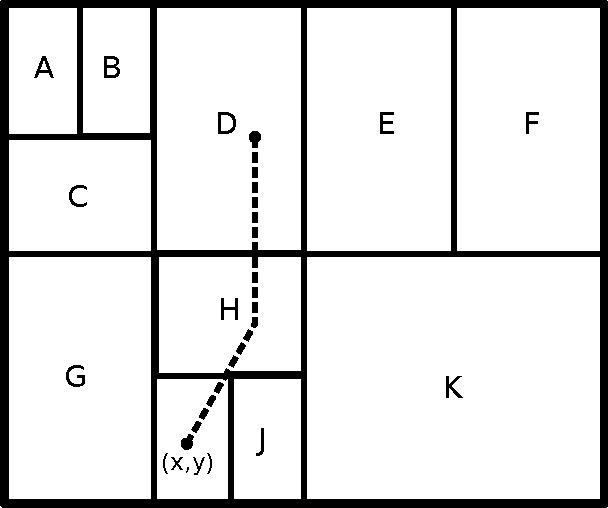
\includegraphics[scale=0.4]{img/algorithms/landmark_binning}
\caption{Example 2D coordinate overlay and a sample routing path from node D to
(x,y).}
\label{fig:landmark_binning}
\end{figure*}

Landmark Binning \cite{ratnasamy_binning_2002} is an approach to partition close
by nodes into bins based on their distance to well known anchor nodes across the
Internet, as shown in Figure~\ref{fig:landmark_binning}. In order to detect
locality, nodes use network latency (i.e. RTT) as a measurement technique. The
network latency, even though not always accurate, is selected in this work due
to its non-intrusive, transparent and easy to apply behaviour. In order for the
binning to work, few well known anchor servers with known physical locations on
the Internet. Authors estimate that a number of 12 such servers can prove
sufficient for this. Every newly arriving node measures its distance from these
landmarks and unilaterally decides to join a specific bin based on these
results. Specifically, the node measures its round-trip time to each of the
landmarks and orders the values in a decreasing order. The ordering represents
a \emph{bin}, in the sence of close-by nodes having the same landmark ordering
and hance belong to the same bin. This means that a landmark system consisting
of $m$ such nodes results in $m!$ potentional different bins.The operation of
the method is independent of the model incorporated by the overlay network and
thus it can be applied with no significant changes to both structured and
unstructured P2P systems. \cite{ratnasamy_binning_2002} has the detailed
description of such algorithm for both architectures. Landmark binning is also
considered as a good candidate for content distribution networks in particular.
The major disadvantage of landmark binning is to install and maintain landmark
servers on different autonomous systems, all over the world. A typical P2P
network usually has a couple of million nodes connected at any given time, thus
rendering landmark servers an important parameter when designing for large
scales.  The authors claim that latency estimation does not drain much from the
network resources but in case scalability problems arise, they claim the
solution is replacing single landmark servers with clusters of servers within
the same physical area. However, this approach does not reduce the possibility
of excessive network traffic flow through these landmark servers. One other
possible problem is the incorrect binning caused by the use of inaccurate
methods for delay measurement, since tracking down, for example, network
latencies is far from proven to be safe for location estimation.

%The algorithm can be considered scalable, as nodes need only compute distances
% to a small number of predefined nodes and thus without exchanging any
%information.
%To answer the question as to whether the algorithm actually contributes
% possitivelly to the construction of an enhaned overlay, the paper defines the
%\emph{gain ratio} as the factor by which the latency reduces when someone
%communicates with a random node from the same bin than with one not in the bin.
%This is implemented with an inter-bin to an intra-bin latency ratio.


%
% TODO: LANDMARK BINING FOR UNSTRUCTURED OVERLAYS
%
%For unstructured overlays the paper assumes \emph{a set of $n$ nodes where each
% node picks any $k$ neighbour nodes so that the average routing latency on the
%resultant overlay is low (assuming shortest path routing)}. According to the
%proposed heuristic algorithm called \emph{BinShort-Long}, a node picks its
%neighbours by choosing its $\frac{k}{2}$ closest\footnote{If the node's bin is
%not large enough for it to pick these $\frac{k}{2}$ neighbours, it picks the
%required nodes from the bin that matches the most in terms of landmark
%ordering.} ones (named \emph{short links}), using the \emph{binning} scheme and
%the rest $\frac{k}{2}$ randomly (\emph{long links}). The former set produces
%well-connected \emph{pockets} of nearby nodes while the later preserves the
%connectivity of the graph, both yielding a proximity factor of $\alpha = 0.5$
%in an attempt to preserve the benefitial properties of unstructured
%topologies\cite{merugu_str2unstr_2003}.

%
% TODO: SOME DISCUSSION
%
%A potential bottleneck could be the extra load that this
%``ping''-like scheme imposes to the landmarks, especially when we need instant
%reaction from our topology when dealing with the dynamic nature of the p2p
%networks.
%
%One disadvantage of this landmark scheme is related to the additional burden
% imposed to the landmark sites. The authors claim though that the algorithm
%requires so little work by the landmarks (maybe just echo to ping messages)
%that could in effect, act as ``unsuspecting participants''. Even if this is the
%case, the fact that it is not fully distributed, renders the protocol's
%scalability directly volnerable to any system size increase as well as
%usuitable for highly dynamic networks such as ad-hoc networks. Moreover, fixed
%points in a network are inherently more exposed to malicius attacks. The most
%significant downside of the algorithm though is that it can lead to an
%extremely uneven overlay ID distribution causing load inbalances and hot spots.
%Lastly, the scheme is coarse grained when it comes to distinguishing relatively
%close nodes\footnote{In the worst case, all nodes could ve clustered into a
%single bin.}.
%

%%%%%%%%%%%%%%%%%%%%%%%%%%%%%%%%%%%%%%%%%%%%%%%%%%%%%%%%%%%%%%%%%%%%%%%%%%%%%%%%
\subsubsection{mOverlay}
\emph{mOverlay} \cite{zhang_moverlay_2004} tries to addresses the scalability
issues that might be imposed to networks (i.e. load unbalance) when using static
landmark servers by introducing dynamic landmarks. Zhang et al. introduce the
notion of a \emph{group} which is a set of peers considered close to each other
with respect to any position in the underlying network, proximity being defined
by some user-defined cost metric like RTT, latency or something else. mOverlay
is considered a clustering approach since it tries to recreate small-world-like
properties to the overlay network by creating a two-level hierarchical
structure, where on the top level we have connections between groups while on
the bottom we have connections between peers inside groups. Finding the correct
closest group is the most important part of the overlay construction. Nodes are
grouped based on their distance to the groups already in the network, rendering
the later the (dynamic) landmarks for the process. The authors formally prove
that any new node can reach its group by exchanging at most $O(logN)$ messages
within the network. Finally mOverlay also considers a second important function
in its protocol which is the constant maintenance of the overlay.

%
%\paragraph{Locating process} A new coming host, $Q$, first connects to a
%globally known host cache called the \emph{rendezvous point (RP)} in order to
%retrieve the starting point in the overlay, say $A$ in group $1$. Host $Q$
%then, measures its distance to host $A$. At the same time, the later, sends
%information about the neighbour groups of group $1$ back to host $Q$. This list
%is called \emph{candidate group list}, and the newcoming host sequnentially
%measures its distance to each of them in seek for the closest one. If the
%\emph{grouping criterion} is met, host $Q$ belongs to group $1$. If not, a boot
%host from the closest group is found and the algorithm is re-run until the
%criterion is met or after a predefined number of repetitions. In the later
%case, $Q$ creates a new group comprising itself only. The above protocol does
%not favour hotspots as it spreads the probability of visiting a group across
%the whole overlay and limits the overhead in the level of $O \left ( log N
%\right )$.
%
%\paragraph{General overlay operations} A set of additional protocols, are also
% introduced, similar to those found in traditional unstructred networks, but
%modified focusing on scalability and robustness. For example a protocol for
%\emph{group formation} is introduced that exploits the inherent characteristic
%of proximity, in the overlay, in order to efficiently detect the neighbouring
%groups of a newly formated group from the set of adjasent groups of its closest
%neighbour. Additionaly, during \emph{group joining} the coresponding protocol
%denotes the exchange of important information for group maintenance. This can
%be furtherly improved by \emph{information sharing} between nodes of the same
%group, functionality handled by a dedicated flood-like protocol\footnote{Since
%nodes that belong to the same group are physically close this can be achieved
%at a minimum price.}. Moreover, another set of distributed protocols handle the
%\emph{information update}. The information that needs update, in the proposed
%architecture, is
%\begin{inparaenum}[\itshape i\upshape)]
%  \item the host cache, when a new node joins, and
%  \item the neighbours of groups, when a close-by group is generated.
%\end{inparaenum}
%Finally, in case of \emph{host failure} or \emph{host departure} the system is
% able to maintain its stability since there are defined operations for
%periodical host cache update and group leader selection if one leaves or dies.
%


%%%%%%%%%%%%%%%%%%%%%%%%%%%%%%%%%%%%%%%%%%%%%%%%%%%%%%%%%%%%%%%%%%%%%%%%%%%%%%%%
%%%%%%%%%%%%%%%%%%%%%%%%%%%%%%%%%%%%%%%%%%%%%%%%%%%%%%%%%%%%%%%%%%%%%%%%%%%%%%%%
\subsection{Discussion on the Algorithms for Unstructured Architectures}
%%%%%%%%%%%%%%%%%%%%%%%%%%%%%%%%%%%%%%%%%%%%%%%%%%%%%%%%%%%%%%%%%%%%%%%%%%%%%%%%
%%%%%%%%%%%%%%%%%%%%%%%%%%%%%%%%%%%%%%%%%%%%%%%%%%%%%%%%%%%%%%%%%%%%%%%%%%%%%%%%



\renewcommand\arraystretch{1.4}% (MyValue=1.0 is for standard)

%\begin{figure}[h!]
\hspace{-3ex}
\begin{center}
\footnotesize
%\begin{tabular}{
%\begin{landscape}
\begin{longtable}{
|>{\columncolor[gray]{.7}}m{0.2\columnwidth}
|>{\columncolor[gray]{.9}}m{0.4\columnwidth}
|>{\columncolor[gray]{.8}}m{0.2\columnwidth}
|>{\columncolor[gray]{.9}}m{0.2\columnwidth}
%|>{\columncolor[gray]{.9}}m{0.1\columnwidth}
%|>{\columncolor[gray]{.8}}m{0.1\columnwidth}
%|>{\columncolor[gray]{.9}}m{0.1\columnwidth}
%|>{\columncolor[gray]{.8}}m{0.1\columnwidth}
|}
\caption{Decentralized Unstructured Algorithms} \label{fig:unstruct_compare_table} \\
\hline
\rowcolor[gray]{.5}
\textbf{Algorithm} &  \textbf{Overlay structure} & \textbf{Base protocol} &
 \textbf{Scalability}\\
\hline
\endfirsthead
\multicolumn{4}{c}%
{\tablename\ \thetable\ -- \textit{Continued from previous page}} \\
\hline
\rowcolor[gray]{.5}
\textbf{Algorithm} &  \textbf{Overlay structure} & \textbf{Base protocol} &
 \textbf{Scalability}\\
\hline
\endhead
\hline \multicolumn{4}{r}{\textit{Continued on next page}} \\
\endfoot
\hline
\endlastfoot
\textbf{Narada} & \textbf{Overlay optimization
based}. Creates a mesh (richer connected graph) and builds minimum spanning
trees on this mesh & & Small and sparse groups \\

\hline
\textbf{Gia} & \textbf{Broadcast based} Replaces
Gnutella flooding with random walk, and introduces KaZaA style supernodes. Uses
dynamic topology adaptation protocol &
 Gnutella &  Better than Gnutella  \\

\hline
\textbf{Adaptive Overlay Topology Optimization} & \textbf{Overlay optimization
based}. Creates overlay multicast tree with Selective Flooding protocol&
Gnutella &  Better than Gnutella \\

\hline
\textbf{Location-aware Topology Matching} &
\textbf{Overlay Optimization Based}. Uses \textit{TTL2-detector flooding}, \textit{low productive
connection cutting}, and \textit{source peer probing}. & Gnutella &  Better than Gnutella \\

\hline
\textbf{Replication Strategies in Unstructured P2P Networks} &
\textbf{Cache Based}. Uses uniform, proportional and square root allocation
strategies to replicate data. & Gnutella &  Better than Gnutella \\

\hline
\textbf{Tracing a large-scale Peer to Peer System: an hour in the life of Gnutella.} &
\textbf{Cache Based}. Proposes a caching algorithm based on the traces of the Gnutella traffic & Gnutella & Better than Gnutella \\

\hline
\textbf{Improving search in P2P networks} &
\textbf{Broadcast Based}. Uses \textit{iterative deepening}, \textit{directed
BFS}, and \textit{local indices} to improve efficiency. & Gnutella &  Better than Gnutella \\

\hline
\textbf{Distributed Cycle Minimization Protocol} &
\textbf{Broadcast based} Uses a decentralized cycle elimination protocol  &  &  \\

\hline
\textbf{Scalable Bipartite Overlay} &
\textbf{Overlay optimization based} Uses bipartite partition graph and builds
local minimum spanning trees  & Gnutella  & Better than Gnutella \\

\hline
\textbf{Adaptive Connection Establishment} &
\textbf{Overlay optimization based} Forms Neighbour Cost Tables, builds local
minimum spanning trees and perform local optimizations & Adaptive Overlay
Topology Optimization (AOTO), Gnutella & Better than Gnutella \\

\hline
\textbf{Hops Adaptive Neighbour Discovery} &  & &  \\

\hline
\textbf{Two-Hop-Away Neighbour Comparison and Selection (THANCS)} &
\textbf{Overlay optimization based} Uses piggybacking to discover neighbour
distances and selects neighbours  & Gnutella  & \\

\hline
\textbf{mOverlay} &\textbf{Landmark based proximity} Uses dynamic landmarks to find node locality
& & Due to dynamic landmarks and grouping, more scalable than tree-based or mesh-based protocols \\

\hline
\textbf{Distributed Domain Name Order (DDNO)} &
\textbf{Overlay optimization based} Connects half of the nodes connections to
the nodes in the same domain and the other half to random nodes, therefore
supports locality and topological connection  &  & Yes, by using super
peers \\

\hline
\textbf{Peer-exchange Routing Optimization Protocols} & \textbf{Overlay optimization based} Optimizes overlay by the exchange of
neighbors among peers  & Can work with both decentralized structured and
unstructured architecture & Yes \\

\hline
\textbf{MAY OMIT - I CHANGED IT TO STRUCTURED SINCE THERE IS A REFERENCE FOR
DHT (OF COURSE IT MIGHT POSIBLE TO BE APPLIED TO BOTH. MAYBE NEED TO CHECK) -
T2MC} &
\textbf{Overlay optimization based} Uses traceroute results for clustering the
nodes  & & \\

\hline
\textbf{Unnamed-unstructured} &
\textbf{Overlay optimization based} Minimizes the communication delay and
maximizes the broadcasting range & & Better than THANCS and mOverlay \\

\hline
\textbf{Landmark Binning} & \textbf{Landmark based proximity} Uses network latency to partition
nodes into bins & Can work with both decentralized structured and unstructured architecture & \\

\hline
%\end{tabular}
\end{longtable}
%\end{landscape}
\end{center}
\vspace{-2.5ex}
\vspace{-2.5ex}
%\end{figure}












%%%%%%%%%%%%%%%%%%%%%%%%%%%%%%%%%%%%%%%%%%%%%%%%%%%%%%%%%%%%%%%%%%%%%%%%%%%%%%%%
%%%%%%%%%%%%%%%%%%%%%%%%%%%%%%%%%%%%%%%%%%%%%%%%%%%%%%%%%%%%%%%%%%%%%%%%%%%%%%%%
\subsection{Discussion on the Algorithms for Unstructured Architectures}
%%%%%%%%%%%%%%%%%%%%%%%%%%%%%%%%%%%%%%%%%%%%%%%%%%%%%%%%%%%%%%%%%%%%%%%%%%%%%%%%
%%%%%%%%%%%%%%%%%%%%%%%%%%%%%%%%%%%%%%%%%%%%%%%%%%%%%%%%%%%%%%%%%%%%%%%%%%%%%%%%


 In short, the methods highlighted here are divided into the following
groups
\begin{inparaenum}[\itshape i\upshape)]
  \item broadcast optimisation
  \item caching,
  \item overlay optimisation, and
  \item landmark -based
\end{inparaenum}
 approaches.

%###############################################################################

%%%%%%%%%%%%%%%%%%%%%%%%%%%%%%%%%%%%%%%%%%%%%%%%%%%%%%%%%%%%%%%%%%%%%%%%%%%%%%%%
%%%%%%%%%%%%%%%%%%%%%%%%%%%%%%%%%%%%%%%%%%%%%%%%%%%%%%%%%%%%%%%%%%%%%%%%%%%%%%%%
\subsection{Broadcast Optimisation} 
%%%%%%%%%%%%%%%%%%%%%%%%%%%%%%%%%%%%%%%%%%%%%%%%%%%%%%%%%%%%%%%%%%%%%%%%%%%%%%%%
%%%%%%%%%%%%%%%%%%%%%%%%%%%%%%%%%%%%%%%%%%%%%%%%%%%%%%%%%%%%%%%%%%%%%%%%%%%%%%%%
% TODO: TAKEN FROM ALGORITHMS SUBSECTION. SHOULD BE MERGED WITH DISCUSSION

In the first realisation of the Gnutella protocol, each query request received
by a peer was then forwarded to all of its neighbours which, clearly, generated
unnecessary traffic over the communication links of all the network. The
algorithms that fall into the group discussed in this section are referred
to as broadcast optimisation -based because they enhance the ``naive''
broadcasting approach, described above, and prefer to forward the messages to a
selected subset of a node's outgoing links. The selection criteria vary
depending on the algorithm but they mainly use one or multiple statistical
metrics that span from some obvious ones, like the latency of the link between
the nodes, to more sophisticated alternatives that may even take into account
application level requirements such as the reliability of the neighbour.
These appoaches have the advantage of enhancing the search responsiveness but on
the other hand suffer from the drastic reduction of the search scope thus
limiting the scalability of the whole network.

%Expanding the search scope, on the other hand, is no easy task
%because the overhead of forming multicast trees is proportional to the
%multicast group size.
%forwarding based schemes do not consider dynamic joining
%and leaving of peers so they do not scale well on dynamic environments.


%###############################################################################

%%%%%%%%%%%%%%%%%%%%%%%%%%%%%%%%%%%%%%%%%%%%%%%%%%%%%%%%%%%%%%%%%%%%%%%%%%%%%%%%
%%%%%%%%%%%%%%%%%%%%%%%%%%%%%%%%%%%%%%%%%%%%%%%%%%%%%%%%%%%%%%%%%%%%%%%%%%%%%%%%
\subsection{Caching}
%%%%%%%%%%%%%%%%%%%%%%%%%%%%%%%%%%%%%%%%%%%%%%%%%%%%%%%%%%%%%%%%%%%%%%%%%%%%%%%%
%%%%%%%%%%%%%%%%%%%%%%%%%%%%%%%%%%%%%%%%%%%%%%%%%%%%%%%%%%%%%%%%%%%%%%%%%%%%%%%%
% TODO: TAKEN FROM ALGORITHMS SUBSECTION. SHOULD BE MERGED WITH DISCUSSION

%\subsection{Cache Based}
%
%Caching based protocols are effectively used to reduce traffic costs and
%response
%times. The caching policy varies depending on the way protocol handles the
%index and the
%content. Centralized P2P systems
%use central index servers, while local caching systems, such as KazaA, use
%super peers
%to cache indices in a distributed way. Content caching is also possible in P2P
%systems, where nodes cache the forwarded content for further retrievals.
%Although caching has the above mentioned advantages,  duplication
%of messages still exist, which limits the scalability of these approaches.
%Therefore, cache based approaches are analyzed in the following categories:
%  \begin{itemize}
%    \item \emph{data index caching},
%    \item \emph{content index caching},
%    \item \emph{centralized}, and
%    \item \emph{local}.
%  \end{itemize}
%
Caching is a widely used technique to exploit locality and minimise redundant
transfer of data, initially adopted by web and file server application
environments with great success. Since peers in a P2P system also work as
servers, it is intuitively expected that P2P file sharing systems can also
benefit from caching. However, two of the main characteristic properties of P2P
systems, nodes frequently joining and leaving and query lifetime relatively
short (at least compared to those needed to be served by web servers) , makes
caching in P2P networks a non-trivial issue. There are usually two levels of
caching possible in file sharing systems, caching indices or pointers to data or
caching the data itself. Caching is already implemented and successfully used in
some commercial P2P systems. One popular example is KazaA, which uses caching of
indices on its super-peer level. In the paragraphs below, caching-based
algorithms are presented and explained in more depth.


%###############################################################################


%%%%%%%%%%%%%%%%%%%%%%%%%%%%%%%%%%%%%%%%%%%%%%%%%%%%%%%%%%%%%%%%%%%%%%%%%%%%%%%%
%%%%%%%%%%%%%%%%%%%%%%%%%%%%%%%%%%%%%%%%%%%%%%%%%%%%%%%%%%%%%%%%%%%%%%%%%%%%%%%%
\subsection{Overlay Optimization}
%%%%%%%%%%%%%%%%%%%%%%%%%%%%%%%%%%%%%%%%%%%%%%%%%%%%%%%%%%%%%%%%%%%%%%%%%%%%%%%%
%%%%%%%%%%%%%%%%%%%%%%%%%%%%%%%%%%%%%%%%%%%%%%%%%%%%%%%%%%%%%%%%%%%%%%%%%%%%%%%%
% TODO: TAKEN FROM ALGORITHMS SUBSECTION. SHOULD BE MERGED WITH DISCUSSION

% These approaches include creating spanning trees using
%connection graphs, creating cluster of physically close nodes, or using latency
%information to detect proximity. The brief description of each category is
%presented below:
%
%  \begin{itemize}
%    \item \emph{Spanning tree based}. These approaches construct of a rich
%    graph  based on the network connections and build minimum spanning tree
%    on the graphs, causing large traffic overhead to the system
%    \cite{chu_esm_2000,chu_esm_2002}.
%
%    \item \emph{Cluster based}. These approaches select to link physically
%    closer nodes with each other, therefore shrink the search scope
%    significantly while mapping accuracy is not always guaranteed.
%
%    \item \emph{Minimum latency first}. Use of latency as a metric to calculate
%    distance among peers. They require global latency information
%    ``landmarks''\footnote{Measuring latency between peers and stable Internet
%    servers.}.
%
%  \end{itemize}

The overlay optimization based protocols modify the topology of the P2P network
using various techniques. The two commonly used approach that is investigated in
this section are creating spanning trees using connection graphs, and creating
clusters of physically close nodes. Spanning tree based approaches construct
rich graphs based on the network connections and build minimum spanning trees on
these graphs. Even though spanning trees provides efficient query performance,
the construction and the update costs of the spanning tree, especially in
dynamic environments with many nodes joining and leaving the network, cause
large traffic overhead to the corresponding
network \cite{chu_esm_2000,chu_esm_2002}. The cluster based approaches on the
other hand select to link physically closer nodes with each other, therefore
significantly shrinking the search scope of the system. Added to that, commonly
used methods for correct determination of physical node positions across
Internet do not always return reliable results, therefore mapping accuracy is
not guaranteed. Bellow, the details of the algorithms that use the spanning tree
based or cluster based topology optimization methods are presented.


%###############################################################################


%%%%%%%%%%%%%%%%%%%%%%%%%%%%%%%%%%%%%%%%%%%%%%%%%%%%%%%%%%%%%%%%%%%%%%%%%%%%%%%%
%%%%%%%%%%%%%%%%%%%%%%%%%%%%%%%%%%%%%%%%%%%%%%%%%%%%%%%%%%%%%%%%%%%%%%%%%%%%%%%%
\subsection{Landmark Based Proximity}\label{sec:landmark}
%%%%%%%%%%%%%%%%%%%%%%%%%%%%%%%%%%%%%%%%%%%%%%%%%%%%%%%%%%%%%%%%%%%%%%%%%%%%%%%%
%%%%%%%%%%%%%%%%%%%%%%%%%%%%%%%%%%%%%%%%%%%%%%%%%%%%%%%%%%%%%%%%%%%%%%%%%%%%%%%%

Detecting the proximity of a node using landmarks, also known as
\textit{Landmark Clustering}, is based on the view that nodes with similar
distances to a set of predefined well-known landmark nodes are pretty likely
being close to each other. But this approach has its weaknesses itself, like the
fact that is a rather coarse grained approximation, therefore not particularly
well suited for detecting the correct positions of nodes within close distance
to each other.


%###############################################################################


In this section we presented the state of the art for the algorithms applied to
unstructured P2P systems. We categorised it based on their philosophy for
alleviating the topology mismatch problem into four major categories namely
\begin{inparaenum}[\itshape i\upshape)]
  \item broadcast-based,
  \item cache-based,
  \item overlay optimisation-based and
  \item landmark-based approaches
\end{inparaenum}
. Here we present a overall discussion on the above categories trying to point
out the advantages, disadvantages and novelties introduced by each and by all of
them. A quick overview can be seen in Table \ref{fig:unstruct_compare_table}.

Broadcast-based approaches in general propose intelligent neighbour selection in
order to replace the inefficient blind flooding first used in the Gnutella
protocol. Instead of forwarding the queries to all their outgoing links they
dictate the intelligent selection of neighbours with either higher probability
to answer a query than others or neighbours  that expose specific features such
as high bandwidth, high capacity, or low latency. This, in practice reduces the
aggregate resource usage of the P2P network and improves the overall performance
of the system. On the other hand, the algorithms do not offer a real solution to
the topology mismatch problem. Thus, none can guarantee that overlay and
underlying topologies are aligned with each other let alone quantify the
mismatch and try to alleviate. Broadcast-based methods can be used in
conjunction with other approaches to improve the quality of the P2P systems.

The success of caching, as a well studied method in client-server Internet
applications, also made it a good candidate for the P2P networks. Even
though caching improves the performance, and reduces the overall resource usage
of P2P systems, the design of caches in this context is non-trivial compared to
the web-based caching. Due to the unique, inherent characteristic of all P2P
systems that, each node can act as both a server and a client, two important
issues have to be considered when designing caches. First, the lifetime of a
query is short, as the nodes join and leave frequently. Second, the result of a
single query string is not always the same, as it is dependent on the source of
the query, the TTL value set for the messages, the current interconnection of
peers and the high volatility of the environment. So, in order to develop a
successful caching system for a P2P architecture, these parameters also have to
be considered. Even though the state of the art P2P algorithms using caching
methods reduce the resource usage of the network, they also fail to consistently
address the probelem of the topology mismatch.

Overlay-optimisation-based  can further be devided into
minimum-spanning-tree-based and clustering-based. Researchers initially started
considering alternatives to IP multicast for the application layer, which led
Narada, that simulates the same one-to-many communication approach requiring IP
multicast services. Application layer multicast, however, is not as efficient as
the one enabled by IP and still struggles to ease the difficulties imposed by
the topology mismatch problem. Narada, and its followers (AOTO, LTM, SBO) try to
solve the topology mismatch problem by building a richer connected graph and
forming minimum spanning trees over this graph that can efficiently route
messages among peers. Application level multicast protocols, pioneered by
Narada, are generic protocols that can be applied to both P2P file sharing
systems, as well as content distribution networks. The original Narada algorithm
is designed for small groups therefore it is not scalable. Its followers try to
solve the scalability problem by introducing various methods including forming
minimum spanning trees for the two-hop neighbours ($N^2$) of each node,
partitioning the graph into two random groups where each group is responsible of
different tasks, or performing local optimizations dynamically on the overlay
graph. The advantage of building minimum spanning trees is that they maintain
the connectivity on the network in an efficient manner, while still preserving
the overall search scope. However, building and maintaining a minimum spanning
tree creates additional overhead for the network. The alternative method used in
overlay optimization is the cluster based approache. According to that, nodes
use various methods to detect physically close nodes to form clusters. T2MC uses
traceroute logs and DDNO uses domain names to cluster close by nodes. However,
the accuracy of the methods used to form clusters directly affect the success
rate of the algorithm. Traceroute for example is a heavy weight utility to be
frequently used on the network, let alone the fact that many network equipment
vendors do not allow traceroute calls. The major problem with cluster based
approaches is that the limited connectivity within the local domains shrink the
search scope dramatically, which negatively affects the search performance of
the P2P system. DDNO addresses this limitation by allowing half of each nodes
connections to be to random nodes over the network, which balances the
efficiency of the clustering approach with improved connectivity.

In landmark-based algorithms, nodes use network delay (e.g. RTT) as a
distance measurement method to position themselves with respect to ``a priori''
known servers (the landmark servers) on the Internet. Landmark servers are used
by nodes to estimate their positions based on the intutive assumption that nodes
with similar distances to a set of landmarks, are physically close to each
other, as well, over the network. The landmark based protocol has two important
drawbacks. Firstly the network delay is not a reliable distance estimation
method. For example, based on the load on the network the delay to certain nodes
or networks can change from time to time, which will eventually affect the
distance measurements and wrong measurements will lead to wrong estimated
positions for the nodes, or incorrect and non optimal clusterings of the nodes.
The second drawback of using landmark servers is the cost of installing and
maintaining this kind of infrastructure across the whole Internet and for all
the different autonomous system domains. As popular P2P file sharing
applications usually have millions of peers connected at any time, it is not
false to assume that the network costs of maintaining these landmark servers
will be quite high. A possible solution to the scalability problem of the static
landmark servers is to use ordinary nodes as dynamic landmarks once they
estimate their own positions. Even though this approach scales much better than
static landmark servers, still the measurement accuracy problem affects the
overall performance of the system.